\documentclass[a4paper,11pt]{article}

\usepackage[margin=1.0in]{geometry}
\usepackage[affil-it]{authblk}
\usepackage{url}
\usepackage{graphicx}
\graphicspath{{figures/}}
\usepackage{todonotes}
\usepackage[titletoc,title]{appendix}

\newcommand{\code}[1]{\texttt{#1}}

\begin{document}

\title{I Came, I Saw, I Planned, I Conquered: \\ A Plan for World Domination}
\author{Jason Gregory, Moshe Katz, \& Kamruzzaman Quddus \\ \{jgregory, mmkatz, kquddus\}@umd.edu}
\affil{University of Maryland, College Park, MD}
\date{\today}

\maketitle

\abstract{In this work, we describe a probabilistic planner that competes in
the Warlight AI Challenge 2.  More specifically, we have implemented and applied the
\emph{Monte Carlo Tree Search} (MCTS) algorithm with the \emph{Upper Confidence Bounds on Trees} 
(UCT) algorithm for winning Warlight games when randomly paired up against users that employ other 
strategies.  Using these probabilistic planners we have successfully won the majority of our games
against random AI bots.}

\section{Introduction}\label{sec:intro}
\subsection{AI in Games}\label{aiingames}
Although there are many major commercial fields that benefit from improvements
in Artificial Intelligence (AI), one of the largest research areas in the field is
the application to games.  From the 1951 debut of artificially intelligent bots
for Nim \cite{nim}, checkers, and chess \cite{checkerschess}, to Deep Blue's 1997
defeat of chess grandmaster Garry Kasparov, and continuing to today's sophisticated
first-person-shooter adversaries, the impact and importance of AI in gaming as a
tool for understanding and furthering AI techniques for application to real-world 
problems cannot be overstated.

Despite all of this work, there still remains many "open problems" in game AI
design.  Many games still use AI bots that are quite naive, and some games have
not yet been determined to be winnable by a computer player. To encourage continued
research and development of game AI, some game makers occasionally run competitions
for developing new AI bots to play their games.

In this work, we have developed a bot to compete in the Warlight AI Challenge 2 
\cite{warlight}. The goal of this competition is to build a bot that can play (and, of 
course, can win) Warlight, a RISK-style game.

\subsection{Warlight} \label{sec:warlight}
For a full discussion of the rules and origins of the game \emph{Warlight}, refer
to our previous paper, \emph{Towards the Planning of World Domination}\cite{ourproposal}.
To recap the major points, Warlight is a game similar to the classic board game RISK, with 
the addition of fog-of-war and randomly-generated maps. The Warlight AI Challenge 2 is a 
competition that pits bots against each other in a series of two-player games and collects 
the scores of the games to determine a winner of the competition.

\section{Related Work}\label{sec:previous}
The largest body of related work is the set of other bots in the current challenge.  
There are currently around 200 competition entries from 30 countries written in 
eleven languages \cite{warlight}.  While we have not examined many of our competitors 
in detail, they are all working toward the same goal as we are of developing an AI bot for 
this game, and some of them are very good at playing the game.

Additional related work comes from the first Warlight AI Challenge.  While the 
rules of the game for that competition were slightly different, many of the 
techniques used there will still apply to this challenge, either as examples of 
successful approaches, or otherwise as examples of what not to try.

There are existing AI bots for the original RISK game.  While some have been 
discussed only theoretically, including strategies from MIT \cite{riskmit}, Markov 
Chains from North Carolina State University \cite{riskncs}, Monte-Carlo (UCT) 
techniques for territory selection from University of Alberta \cite{riskalb}, and 
studies of dice-rolls from Elon University \cite{riskelon}, implementations of AI 
players for RISK have been created and sold in commercial software as early as 1989. 
These solutions are also of varying quality - the 1992 release of \textit{WinRisk} for 
Windows 3.1 was capable of beating at-best an inexpert child player - and most 
implementations are closed-source without any documentation of their algorithms.

The UCT algorithm has been used as the basis for other games: the algorithm was originally 
described for the game \emph{Go}\cite{uct}, then also applied to 
\emph{backgammon}\cite{uctback}.  However, unlike Warlight, in both of those games, the game 
itself is played on a board of finite size and both players have full knowledge of the state 
of the board.  In contrast, Warlight's random maps mean that we cannot know anything about 
the board size and layout beforehand, while Warlight's for of war means that we do not have 
perfect knowledge of the board. UCT has also been used for more complex games, such as 
Tantrix\cite{tantrix} which has a much more dynamic board than Go and backgammon.

\section{Approach}\label{sec:approach}
We have built a bot that uses \emph{Monte-Carlo Tree Search} (MCTS) and \emph{Upper 
Confidence Bound for Trees} (UCT) to play Warlight.  We have also built an ``Opponent Bot'' 
that performs its moves greedily instead of using our algorithm.

\subsection{MCTS}
While traditional AI algorithms for playing games rely on static evaluation functions that 
analyze the game tree to determine the next move to make based on the current state of the 
game, Monte-Carlo Tree Search uses an entirely different approach.  Taking into account that 
the game tree of complex games may be too big to analyze completely for every move, MCTS 
uses a cycle of \emph{Selection, Expansion, Simulation, and Back-Propagation} to build and selectively 
explore the game tree, as shown in Figure~\ref{fig:mcts_alg}, \cite{mcts}.  At a high level, MCTS randomly 
samples the search space within a game by simulating particular branches of the game tree to arrive at 
a plan.  These are referred to as a Monte Carlo rollout policy. As MCTS simulates and evaluates the 
branches of the game tree, the algorithm iteratively adds new states from which it can plan over.  
It is important to notice the distinction between these planning states, which MCTS creates based on 
simulations, and the states of the game, which are generated by the game engine as a result of executing 
moves.  The MCTS algorithm starts its planning process based on the game engine's state, i.e. actor's 
state, and produces new states that could come true if a particular action were taken.

%
\begin{figure}[!htbp]
  \centering
  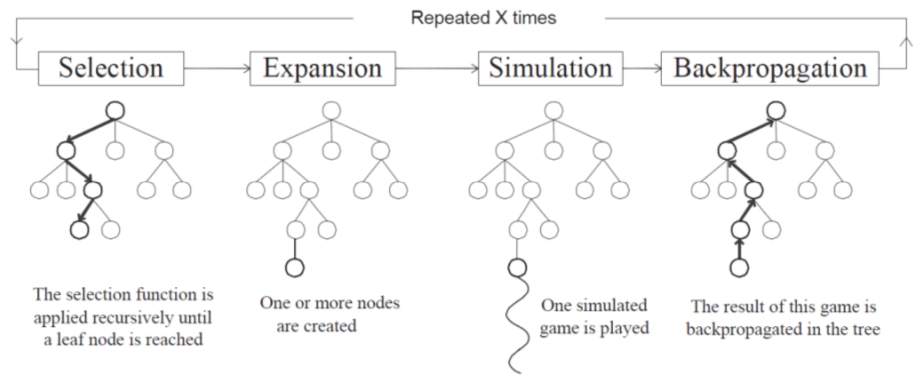
\includegraphics[width=0.7\columnwidth]{mcts_algorithm}
  \caption{The MCTS algorithm used in this work \cite{mcts}.}
  \label{fig:mcts_alg}
\end{figure}
%

\subsubsection{Selection}
The first step of MCTS is finding a node of the game tree from which to further 
analyze.  The choice of which node will be selected must balance the two goals of 
\emph{exploration} and \emph{expansion} -- whether to strike off in a new direction in the 
tree to see if the result will be better or to press farther down the current path.

Within the MCTS ``Selection'' step, we use UCT to determine the ideal node for 
selection.  We apply the UCT algorithm on the existing game tree to determine a score for each node, 
then choose the node with the best score.  For information about the UCT algorithm, see Section~\ref{sec:uct}.

\subsubsection{Expansion}
Once a node has been selected, the Expansion process begins. For this, 
the algorithm computes a random move, generates the resulting state by simulating the random move, 
and adds this new node to the game tree. The random move could consist of doing nothing or any 
number of attacks and transfers between regions.  Additional detail on our approach for generating
a move is described in Section~\ref{sec:move_gen}.

\subsubsection{Simulation}
After a single node is added, a game of alternating turns between the user's bot and an 
opponent bot is simulated starting from the state of the node created in the Expansion step.  
%We use our OpponentBot (described in section \ref{sec:oppbot}) to simulate the opponent's moves 
%during this step.  
Each player generates a random move, which is then simulated to produced a new resulting state.
To simulate a move, we copied the battle simulation code directly from the open-source game engine
to ensure our results were as probabilistically correct as possible. In terms of generating moves
for the opponent, we first used a StarterBot, which is the baseline code that the competition 
organizers initially provide.  In an attempt to improve our implementation of MCTS, we developed 
a more sophisticated OpponentBot, described in Section~\ref{sec:oppbot}.  The implementation of the
OpponentBot is deliberately simple -- simpler than our primary planning algorithms -- in order to 
leave the bulk of our limited execution time for the MCTS and UCT operations.  Note, due to time 
restrictions imposed by the game engine, we currently simulate approximately 10 turns and then stop.  
Provided we have extra time during the game, we could simulate more iterations to gain additional
 knowledge about the path we are taking.

\subsubsection{Back-Propagation}
After a simulation is complete, the node at which the simulation was executed, and all of its 
ancestors in the tree, are updated with a measure of how successful traversing this branch was 
for our bot. Since we do not always simulate to the end of a game, we cannot simply use the measure
of whether the game was a win, loss, or draw.  In the event, the branch we traversed resulted in a win
or loss, we certainly must use this information; however, we did not rely on simulating to this point
in order to evaluate moves. In fact, we developed several metrics for which to evaluate
the quality of a branch in the game tree.  Of these, the most successful were 1) the ratio between 
the number of regions the user bot owns and the total number of regions in the game and 2) the 
ratio between the number of regions the user bot owns  and the number of regions we believe the 
opponent owns.  Ultimately, we used the first metric because of its ability to capture growth of 
power and because of its simplicity to calculate.  

%record of whether that game was a win, a loss, or a draw.  
%This information is used by UCT in the future rounds' selection steps.

\subsection{UCT}\label{sec:uct}
The UCT algorithm provides an efficient method for sampling the search space of the game tree and 
determining where the MCTS algorithm should focus its planning efforts. To balance the need for 
exploration of entirely new paths through the game tree with exploitation of known paths, the UCT 
algorithm maintains an exploration bias that grows over time, as well as a performance score for each node. 
This performance score relates how much a particular action contributes to winning a game.
We implemented this algorithm exactly as shown in the pseudo code provided in Figure~\ref{fig:uct_alg}, 
\cite{Nau2015}, \cite{NauLecture}. Here $n(s)$, $n(s,a)$, and $n(s,\tilde{a})$ correspond to the number of 
times the UCT algorithm has visited a particular state, which contributes to the calculation of the 
exploration bias, $(\frac{log(n(s))}{n(s,a)}^{\frac{1}{2}})$. In our implementation, we chose a weighting 
factor, $C$, of value $2$ to replicate the objective function used in the Upper Confidence Bound (UCB) 
algorithm, which UCT is derived from. Finally, the $Q(\cdot, \cdot)$ value is the performance score for
a given (state, action)-pair.  This provides the functionality of exploiting actions that lead to more 
favorable states.

%
\begin{figure}[!htbp]
  \centering
  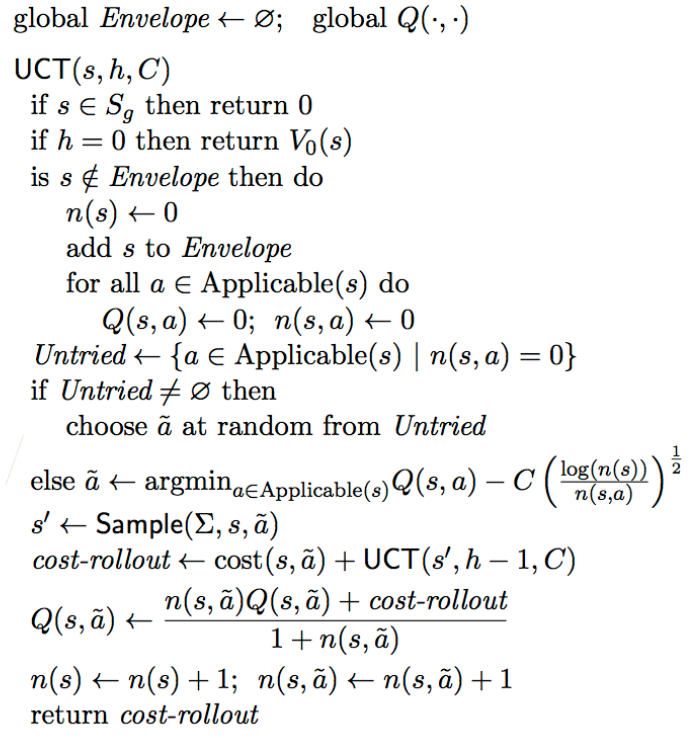
\includegraphics[width=0.45\columnwidth]{uct_algorithm}
  \caption{The UCT algorithm used in this work \cite{Nau2015}, \cite{NauLecture}.}
  \label{fig:uct_alg}
\end{figure}
%


\subsection{Random Move Generation}\label{sec:move_gen}
The generation of moves for MCTS consists of either choosing to do nothing, attacking a neutral 
or enemy region, or transferring troops to an already-owned region. The overall performance of 
MCTS and UCT appears to rely heavily on the quality of random move selection and, while we want to
explore the full spectrum of actions, we also want to ensure we are only evaluating moves that are
sensible to increase our chances of winning. As a result, we explored several options for the 
generation of random moves. Intuitively, our first implementation of simulating a move involves total 
randomness.  That is, we randomly select a single region that we own, randomly select one of its 
neighbors, and issue a command to send all of the owned region's troops to the neighboring state.  
If the neighboring region also happens to be owned by our bot then this simply results in a transfer 
of troops; however, if the neighboring region is neutral or owned by the opponent we will attack it. 
In some instances, this results in needless transfers or, in the worst case, a region with a small 
number of troops attacking a neighbor with a large number of troops, which are very undesirable 
characteristics. 

The second approach we took to move generation improves this technique slightly by selecting one of 
our regions that has the largest number of troops and attacking or transferring to a random neighbor.  
This modification increases the probability of executing an intelligent action, but still leaves room 
for improvement.

Our third implementation of random move generation consists of sorting all of our owned regions
by the number of troops in a decreasing order and, for each owned region, searches for a neighboring
region that we do not own. This ensures that our region with the largest concentration of troops will
always attack a neighboring region. While this approach removes the unnecessary transfers between 
already-owned regions, it also removes all transfers, which could be undesirable late in the game
when a transfer could help a region survive an attack. 

Our fourth, and final implementation of move generation, provided a monumental improvement.  The 
approach is as follows: for every region that we own and has at least 3 troops, sort its neighbors 
by decreasing number of troops, and find the neighboring region that we do not own and has the smallest
 number of troops. If there exists no eligible, neighboring region, simply transfer to the region with 
the smallest number of troops.  If there is, however, a neighboring region that we could attack, we 
quickly evaluate whether this is  an intelligent action.  More specifically, if our region has less 
than or equal to the number of troops in the neighboring region, we refrain from attacking.  If our 
region has approximately 1.5 times the number of armies as the neighboring region then we attack with 
that many troops as this is probabilistically the number of troops required for a successful attack. 
Finally, if we do not have 1.5 times the number of troops as the opposing region, we attack with all 
of our troops to maximize success. This approach has several enticing properties.  First, and 
foremost, we iterate all of our owned regions and compute an attack or transfer.  These results are 
concatenated together and provided to the game engine so that we perform any number of attacks or 
transfers in a single move.  The addition of multiple moves per turn appears to be the largest 
contributing factor in terms of overall performance and winning games. A second desirable 
characteristic of this approach is that it efficiently evaluates the quality of an attack before blindly
executing it.  This eliminates all unfavorable attacks and balances the number of transfers. 
Additionally, by calculating how many more troops our region contains than the opposing region, we 
ensure that we only attack with what we believe to be the minimum number of troops.  From this, our bot
maximizes the probability of a successful attack, while still leaving troops that are unnecessary for
the attack in their original region so that they can provide support for defending.

\subsection{Opponent Bot}\label{sec:oppbot}
Most existing UCT literature and applications simulate both the AI player's and opponent's
moves, requiring complete visibility of the current state of the game; an expectation that
is often taken for granted by MCTS and UCT algorithm designers. However, in the Warlight 
Challenge, the only visibility UCT-based bots have is the regions which are immediately 
adjacent to its owned regions on the board. To compensate for the added complexity of 
implementing UCT with imperfect knowledge, a separate bot class called ``OpponentBot'' is 
designed to mimic the behavior of the opponent and thus work around the lack of full game 
board visibility.

The OpponentBot is designed as a greedy, depth first search-like algorithm with constraints 
(troops per turn, defined number of regions it owns and can operate within) and the requirement 
to be as run-time inexpensive as possible. Given its current list of regions, the algorithm calculates
the cost of obtaining super regions given its present state and prioritizes its plan of
region acquisition accordingly. The plan is adjusted each turn given the known state of the 
game at that turn. Because the DFS algorithm is meant to be an approximation of what an
actual opponent might have been doing both behind the `fog of war' and within visible area, 
its internal hypothetical state must be regularly updated with the actual state changes
provided by the game engine.  The update mechanism operates via internal state recalculations 
triggered by event handlers listening to game engine broadcast messages. While the
opponent bot algorithm was intended to complement our implementation of UCT, we have found 
that it may yet be robust enough to be a stand-alone bot agent. By estimating how a real 
opponent might behave, it allows us to maintain the classic model of UCT, including the 
assumption of full knowledge of the game.

\section{Implementation}\label{sec:impl}
Our bot is implemented in C++, and the code is publicly available on Github\cite{github}.  
The bot takes input on \code{STDIN} and returns commands to be executed back to the game 
engine on \code{STDOUT}.  All of the algorithms (MCTS, UCT, and the Greedy OpponentBot) are 
implemented in classes in the code base, the first two in a class called \code{MCTSManager} 
and the latter in \code{OpponentBot}.  Additional classes are included for parsing the text 
input from the game engine and for storing the state of game play.  The input parser, basic 
outline of the bot code, and the classes for watching the bot state are all based on the 
starter code provided by the Warlight developers, referred to as StarterBot.  In an effort
to focus on the algorithms, we chose to use a tree structure library called \emph{tree.hh}\cite{treehh}.
As it was the primary objective for this work, we have included screen shots of our UCT
implementation in Appendix A.


\section{Experiments}\label{sec:experiments}
The simplest experiment for our bot was to submit it to the challenge server and see how it 
fared against other bots.  We have tested our bot against multiple other bots participating 
in the challenge, and at the time of writing this report we have won 17 out of 20 games.  
Of those 20 games, we had 2 ties and only 1 loss. It is important to note, however, that
some of this success is due to the fact that some people may have uploaded incomplete bots or 
simply unmodified StarterBots, and these results may not be fully representative of our performance.

We are building an experiment in which we pit our MCTS/UCT bot against our greedy 
OpponentBot to determine how much better we can do with the intelligent bot than the greedy 
one.  However, we do not yet have results of this match. Currently, the greedy agent performs 
well as a stand-alone agent in test environment independent of UCT; however it is currently 
still going through some integration issues with  UCT. Originally developed to be run-time 
inexpensive so that the UCT implementation might make the most of pre-allocated runtime 
constraints imposed by game engine, the greedy algorithm was not designed with the design 
flexibility of modern object oriented language and was more tightly coupled by multiple 
container stacks and synchronizing event handler type routines. Thus complete integration 
of state classes employed by parent UCT algorithm is taking a little more time than expected 
and remains a work in progress. However tangential the development of the DFS algorithm might 
have been within the scope of an UCT algorithm, the appeal of developing complementary planning 
algorithm as an academic exercise was simply too appealing to ignore.

For an initial evaluation of our MCTS with UCT implementation, we submitted our bot to the game 
engine and collected the results from 11 different games when matched against the website's test 
bot. We repeated the same process for a primitive bot that we developed earlier in this work.  
This primitive bot selects the region that has the largest concentration of troops and attacks 
or transfers all of its troops except for one to a randomly-selected neighbor. The results of 
11 trials for both of these two bots are summarized in Tables~\ref{tab:primitive_results} 
and~\ref{tab:uct_results}.

%
\begin{table}[!htbp]
  \scriptsize
  \centering
  \begin{tabular}{|c|c|c|c|c|c|}
    \hline
    \emph{Game Number} & \emph{Total Turns} & \emph{Win/Loss/Tie} & \emph{End Turns} & \emph{Regions Captured} & \emph{Super Regions Captured} \\
    \hline
    1   & 60 & T & 60 & 12/21 & 0/4 \\
    2   & 60 & T & 60 & 12/21 & 1/6 \\
    3   & 60 & T & 60 & 10/17 & 1/4 \\
    4   & 60 & T & 60 & 16/20 & 3/5 \\
    5   & 60 & T & 60 & 12/18 & 2/6 \\
    6   & 60 & T & 60 & 20/22 & 4/6 \\
    7   & 60 & T & 60 & 13/21 & 2/5 \\
    8   & 60 & T & 60 & 5/19 & 1/4 \\
    9   & 60 & T & 60 & 4/18 & 0/4 \\
    10  & 60 & T & 60 & 12/18 & 1/4 \\
    11  & 60 & T & 60 & 15/19 & 3/5 \\
    \hline
  \end{tabular}
  \caption{Results for the primitive algorithm that selects the largest concentration of troops and attacks or transfers to a random neighbor.}
  \label{tab:primitive_results}
\end{table}
%

%
\begin{table}[!htbp]
  \scriptsize
  \centering
  \begin{tabular}{|c|c|c|c|c|c|}
    \hline
    \emph{Game Number} & \emph{Total Turns} & \emph{Win/Loss/Tie} & \emph{End Turns} & \emph{Regions Captured} & \emph{Super Regions Captured} \\
    \hline
    1   & 60 & T & 60 & 17/18 & 5/6 \\
    2   & 60 & T & 60 & 16/20 & 5/6 \\
    3   & 60 & T & 60 & 21/22 & 5/6 \\
    4   & 60 & W & 59 & 16/16 & 4/4 \\
    5   & 60 & W & 56 & 19/19 & 5/5 \\
    6   & 60 & T & 60 & 20/22 & 4/6 \\
    7   & 60 & W & 28 & 22/22 & 6/6 \\
    8   & 60 & W & 54 & 19/19 & 6/6 \\
    9   & 60 & T & 60 & 18/20 & 4/5 \\
    10  & 60 & T & 60 & 14/17 & 3/4 \\
    11  & 60 & W & 48 & 19/19 & 6/6 \\
    \hline
  \end{tabular}
  \caption{Results for the MCTS with UCT algorithm.}
  \label{tab:uct_results}
\end{table}
%

\section{Conclusion}\label{sec:conclusion}
From the results show in the tables of Section~\ref{sec:experiments}, we make several observations. 
First, as one would expect, the primitive bot fails to win a single game.  While the primitive bot
does not actually lose any games, it provide no planning for either its actions or the opponent's 
actions and executes a large number of unnecessary transfers that ultimately wastes turns and 
decreases efficiency in obtaining regions. At the end of these 11 trials, the primitive bot owned
on average $61.2\%$ of the regions and $34.0\%$ of the super regions.

The MCTS with UCT algorithm, on the other hand, has a much more focused approach to attacking and 
transferring through its more sophisticated planning technique. As a direct result of sampling the 
search space for improved actions, the MCTS with UCT algorithm is able to win 5 of 11 games.  In the
remaining 6 games that it tied, it owned an average of $89.1\%$ of the regions and $78.8\%$ of the 
super regions. The MCTS with UCT algorithm clearly was more efficient at executing moves due to the 
addition of planning and it is not hard to imagine that this bot would have eventually won the 
remaining 6 games, if allowed a small number of additional turns.

Additionally, through our testing, we have determined several other general characteristics of our 
implementation.  First, we bring to light the importance of our application, namely that our bot 
is competing against other AI bots. From visual inspection of several games, one immediately observes 
the poor performance of most bots submitted to the competition. This factor plays an important role
in our implementation.  We found that the specific strategy for attacking and transferring troops
appears to be more impactful than the addition of MCTS and UCT.  We believe this is because the states 
we are planning over have such large amounts of variance from the eventual game states.  This is 
either due to the uncertainty introduced by fog of war or the misrepresentation of predicted opponent
moves. In our efforts, we believe we may have developed an opponent bot that is overly complicated
and takes more into consideration than that of our opponent's AI implementation. Likewise, in the
beginning of the game, we know virtually nothing about the opponent so attempting to predict their
moves when we don't know the regions they own is nearly impossible. We offer that it may make sense
to have an adaptive planning depth where we simulate deeper into the game as the game progresses into
later rounds and there is more certainty of the overall environment.  Considering all this, we 
hypothesize that the MCTS with UCT algorithm would be more useful and demonstrate its value more 
effectively if it were competing against a human player where the opponent is much more intelligent 
and predicting their moves, while more complicated, may be more feasible.  We believe, this would be 
especially true later in the game when there is less fog of war and more certainty about where the 
opponent has a presence.

\bibliographystyle{plain}
\bibliography{references}

\newpage

\begin{appendices}
\section{Implementation Screen shots}
Figures~\ref{fig:uct_imp} and~\ref{fig:uct_helper_imp} provide screen shots of the C++ source code
that implements the UCT algorithm, as described in Section~\ref{sec:uct}.

%
\begin{figure}[!htbp]
  \centering
  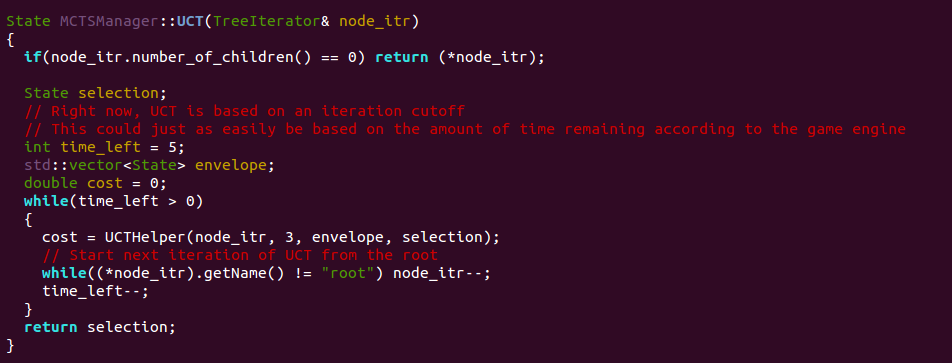
\includegraphics[width=0.71\columnwidth]{uct_implementation}
  \caption{The UCT function definition that repeatedly calls the UCTHelper function as long as time permits.}
  \label{fig:uct_imp}
\end{figure}
%

%
\begin{figure}[!htbp]
  \centering
  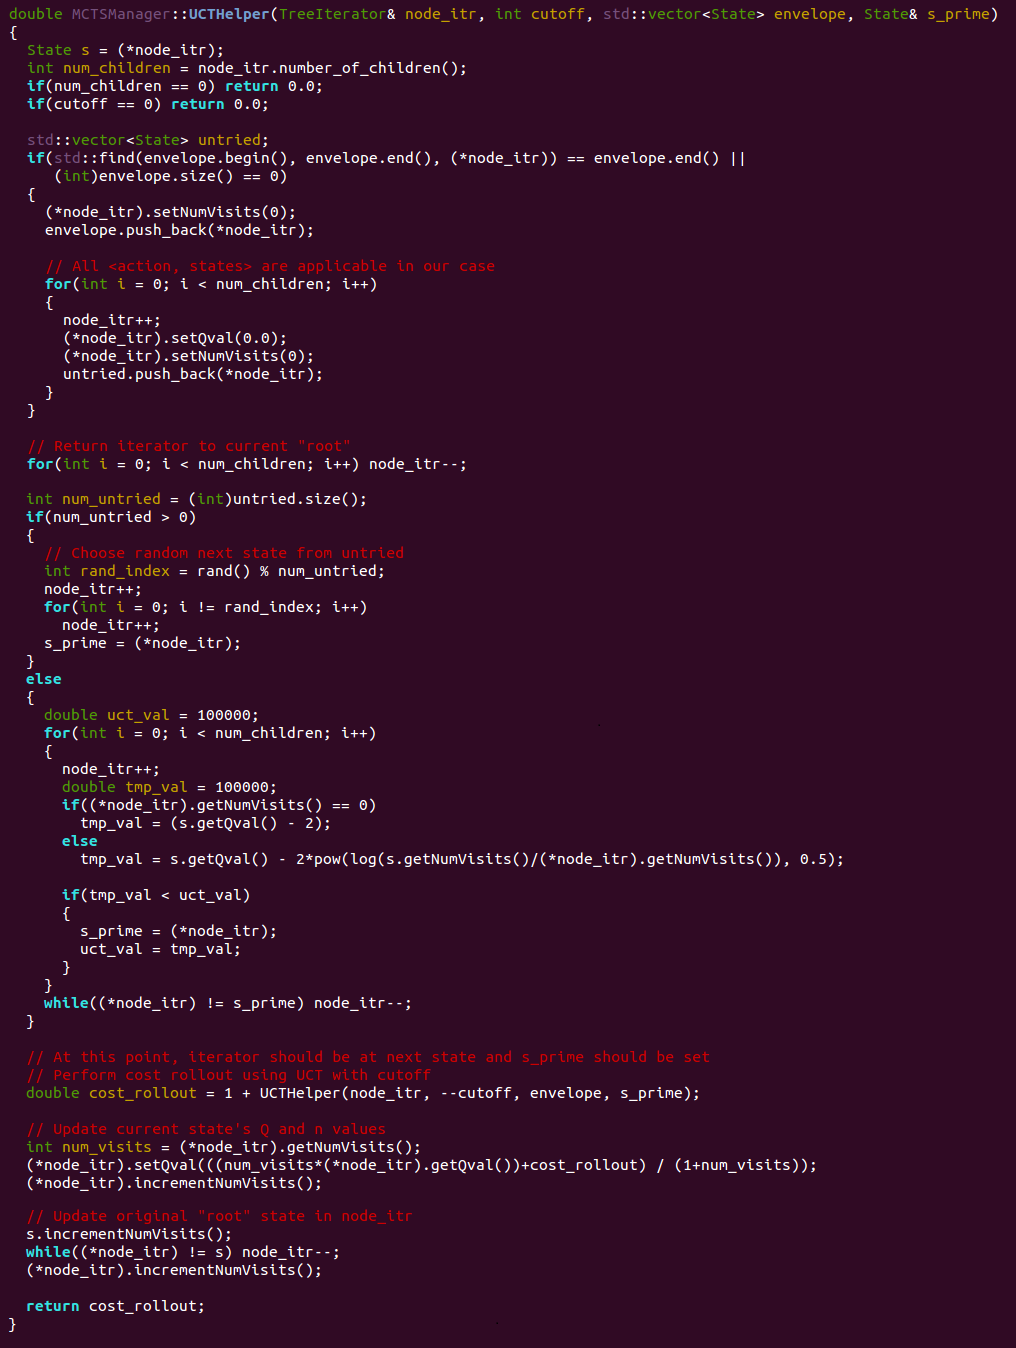
\includegraphics[width=0.71\columnwidth]{uct_helper_implementation}
  \caption{The UCT helper function that implements the pseudo code shown in Figure~\ref{fig:uct_alg}.}
  \label{fig:uct_helper_imp}
\end{figure}
%



\end{appendices}



\end{document}
